\chapter{Design and Implementation}
\label{chap:implementation}
\todo{...fill me...}

\section{Design and Implementation of the Context Broker}
\label{sec:broker}
This work first implements a regular Context Broker, with no fault tolerance resources. Then, it proposes a strategy to give the Broker High Availability function.
 
\subsection{Platform Choice}
The programming language chosen for the development of this work was Python. 

The system was implemented over a HTTP REST (Representational State Transfer) Interface. A REST Interface is \cite{fielding2002principled}. For the RESTful implementation, Python Flask framework was used \cite{flask}. For the created web interfaces, \cite{bootstrap} was used.

For data persistence, MongoDB was used.

\subsubsection{Python, PyCharm and GitHub}
Python is a powerful and easy to learn modern programming language \cite{python}. It was chosen because it represents a challenge, and to show that the system is independent of the programmed language, i.e. different applications developed on different programming languages can interact with each other in the architecture, the messages exchanged are what matters. The Python IDE \cite{pycharm} was used, along with GitHub for version control \cite{github}.

\subsubsection{Flask}
\todo{...brief explanation of Flask...}
\subsubsection{MongoDB}
\todo{...brief explanation of MongoDB and NoSQL...}


\subsection{System Architecture}
In Figure \ref{fig:diagram} an overall diagram of the system is illustrated. Each node is a component of the system, and the arrows represent the interactions between them.

\begin{figure}[h]
	\centering
	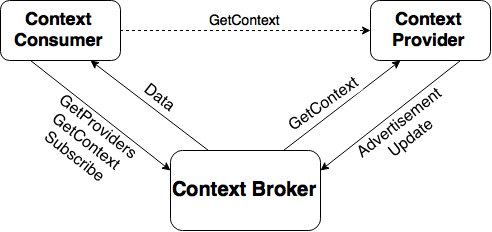
\includegraphics[scale=0.5]{diagram.png}
	\caption{Architecture diagram}
	\label{fig:diagram}
	
\end{figure}


\subsection{Broker Interfaces}
The Context Broker implements several interfaces for communication with the other system components. This section presents each interface and the way they were implemented: what they expect as input (HTTP request from Consumer or Provider), the action they perform, and what they provide as output (response to the Consumer or Provider).


\subsubsection{Advertisement}
\begin{itemize}
	\item[Input:] an Advertisement ContextML message, with Provider information
	
	\item[Action:] registers the Provider within the Broker
	
	\item[Output:] responds the Provider with a ACK or NACK ContextML message, informing success or error, with the corresponding error message.
\end{itemize}

\subsubsection{Update}
\begin{itemize}
	\item[Input:] a ctxEl ContextML Message, with context information to be registered in the Broker
	
	\item[Action:] registers in the Registry Table the context information, with its \textit{contextProvider}, \textit{scope} and \textit{entity} information, \textit{timestamp} and expiration date (\textit{expires}) of the information. It also checks if a \textbf{Subscription} exists for the updated information, sending it to the Consumer \textit{callbackUrl}, when applied.
	
	\item[Output:] responds the Provider with a ACK or NACK ContextML message, informing success or error, with the corresponding error message.
\end{itemize}

\subsubsection{Get Providers}
\begin{itemize}
	\item[Input:] \textit{scope} (mandatory) and \textit{entity type} (optional) arguments in the URL
	
	\item[Action:] looks for registered Providers that provide information matching the arguments given
	
	\item[Output:] responds the Consumer with Providers Lookup ContextML message, containing a list of the providers that match the requested arguments
\end{itemize}

\subsubsection{Get Context}
\begin{itemize}
	\item[Input:] from the Consumer, arguments \textit{scope} and \textit{entity} in the URL
	
	\item[Action:] looks for the latest Context information in the registry that matches the entity and scope received
	
	\item[Output:] responds the Consumer with a ctxEls ContextML message, containing the , or with a NACK ContextML message, informing the error.
	
\end{itemize}
* As seen in Figure \ref{fig:diagram}, there can also exist a direct \textit{GetContext} request from the Consumer to the Provider, thus not involving the Broker. This can be done by the Consumer asking the Broker for a providers list regarding a certain \textit{scope}, and then asking it directly for the desired context information. 

\subsubsection{Subscribe}
\begin{itemize}
	\item[Input:] arguments as follows:  \textit{callbackUrl}, with the URL to where the Broker sends the content it is subscribed to; \textit{scope} and \textit{entity}, with corresponding information the consumer wants to subscribe to; and \textit{minutes}, with the amount of time, in minutes, that the subscription is valid.
	
	\item[Action:] registers the subscription
	
	\item[Output:] responds the Provider with a ACK or NACK ContextML message, informing success or error, with the corresponding error message.
\end{itemize}

\section{UML representation}
The interactions between the clients (Consumers and Providers) and the server (Broker) will be presented using the Unified Modeling Language, UML \cite{uml}.

\subsection{Use Case Requirements}
To present the Use Cases, a list of requirements is provided below. These requirements are adapted from a previous work \cite{crippa2010}, to the functions of this work.

\begin{enumerate}
	\item Register of Context Providers 
	\begin{description}
		\item (a) Receive Advertisement message 
		\item (b) Register CxP on Providers Table
	\end{description}
	\item Context Providers Lookup
	\begin{description}
		\item (a) Receive Providers Lookup request (GetProviders)
		\item (b) Answer with requested Providers data
	\end{description}
	\item Subscribe Context Consumer to data  
	\begin{description}
		\item (a) Receive Subscription request
		\item (b) Register Subscription on Subscriptions table
	\end{description}
	\item Context data interactions  
	\begin{description}
		\item (a) Receive Context data from a Context Provider (Update)
		\item (b) Send Context data to subscribed Consumers
		\item (c) Receive Context data request from a Context Consumer (GetContext) and respond
	\end{description}
\end{enumerate}

Both \textbf{Lookup} and \textbf{Register of Context Providers} services makes the Broker aware of the existence of Context Providers in the network. These are basic duties of a broker in SOA \todo{(find a reference, or take it out; also add SOA to abbreviations)}

The rest of the requirements deal with context data provision and querying, by Providers and Consumers. The Providers see the Broker as the component where they send their context information, so Consumers can find and interpret it. The Consumers see the Broker as the centralized point from where to get up-to-date context data.


\subsection{Use Cases}
When a request from outside the system is received, the behavior is described in a \textbf{Use Case} \todo{(find a reference that defines it)}. In this work, the actors are the Context Broker, the Context Provider and the Context Consumer. The following list presents the use cases in the system. For the sake of brevity, the word "Context" will be omitted when referring to the actors.

\subsubsection{Register of Providers}
\begin{itemize}
	\item[\textbf{Name}:] Register Provider
	\item[Actor(s):] Provider, Broker
	\item[Objective:] Register Provider from an Advertisement ContextML message received from it
	\item[Description:] Validates the ContextML message against the ContextML schema, then registers the Provider and its capabilities (e.g. scopes and entity types it covers) in the Broker 
	\item[Type:] Primary and Essential
	\item[References:] Requirements 1.a, 1.b 
	\item[Sequence of Events:]\hfill
		\begin{enumerate}
			\item Provider sends Advertisement ContextML message to the Broker
			\item The Broker receives and validates the message
				\begin{itemize}
					\item If not valid, the Broker sends a NACK ContextML message to the Provider
					\item If valid, the Broker registers the Provider if new, or updates its information if already existent. If there is an error during the process, a NACK ContextML message is sent to the Provider.
				\end{itemize}
			\item  \todo{what about the timer?}
			\item The Broker sends an ACK ContextML message to the Provider, the registration was successful
		\end{enumerate}
\end{itemize}

\subsubsection{Provider Lookup service}
\begin{itemize}
	\item[\textbf{Name}:] Receive Provider Lookup request
	\item[Actor(s):] Consumer, Broker
	\item[Objective:] Receive, validate and find Providers that match the arguments received from the Consumer
	\item[Description:] The Broker is the only component of the system that has information about all the Providers, thus if a Consumer wants to know where to find a specific information (matching a particular scope or entity), it must ask the Broker for a list of Providers that provide this information.
	\item[Type:] Primary and Essential
	\item[References:] Requirement 2.a 
	\item[Sequence of Events:]\hfill
	\begin{enumerate}
		\item Consumer sends a GET HTTP message to the Broker's \textit{getProviders} interface, with \textit{scope} and \textit{entity type} arguments in the URL.
		\item The Broker validates the arguments: the scope argument is mandatory, while the entity is optional
		\begin{itemize}
			\item If the scope argument is blank, the Brokers responds to the Consumer with a NACK ContextML message, informing the "Bad Parameter" error, in the error message
			\item If the scope is valid, the Broker searches at its internal information for the Providers that match the requested scope and entity type
		\end{itemize}
		\item The Respond Provider Lookup request is started
	\end{enumerate}
\end{itemize}

\begin{itemize}
	\item[\textbf{Name}:] Respond Provider Lookup request
	\item[Actor(s):] Consumer, Broker
	\item[Objective:] Respond to the Consumer a list of Context Providers that match the information requested (\textit{scope}and \textit{entity type})
	\item[Description:] The Broker creates a Providers Lookup ContextML message with the information of the Providers that match the search criteria, and sends it to the Consumer
	\item[Type:] Primary and Essential
	\item[References:] Requirement 2.b 
	\item[Sequence of Events:]\hfill
	\begin{enumerate}
		\item The Broker creates the Providers Lookup ContextML message with the desired Providers. If no Providers match the search criteria, a NACK ContextML message is created, informing "No results found" in the error message
		\item The resulting message is sent to the Consumer
	\end{enumerate}
\end{itemize}

\subsubsection{Subscribe Consumer to data}
\begin{itemize}
	\item[\textbf{Name}:] Register Subscription from Consumer
	\item[Actor(s):] Consumer, Broker
	\item[Objective:] Register a Subscription made by a Consumer, to a certain \textit{entity id}, \textit{entity type} and \textit{scope} combination
	\item[Description:] The Subscription system provided by the Broker is a way of a Consumer to receive any new context information as soon as it is received by the Broker, within a given entity and scope combination. The Subscription is valid for a certain amount of time, defined by the Consumer. The Consumer also informs the Broker a callback URL, to where the Broker sends the new context information the Consumer is subscribed to.
	\item[Type:] Primary and Essential
	\item[References:] Requirements 3.a, 3.b 
	\item[Sequence of Events:]\hfill
	\begin{enumerate}
		\item The Consumer sends a POST HTTP message to the \textit{subscribe} interface of the Broker, with \textit{entity}, \textit{scopeList}, \textit{callbackUrl} and \textit{minutes} arguments in the URL
		\item The arguments are validated, 
		\begin{itemize}
			\item If any is blank or the minutes value is less than one (1), a NACK ContextML message is sent to the Consumer
			\item If all arguments are valid, the Broker checks if the information given in the arguments exists within the Broker. If not, a NACK ContextML message is sent to the Consumer
		\end{itemize}
		\item The Subscription is registered in the Subscriptions table in the Broker
		\item \todo{what aboute the timer?}
		\item An ACK ContextML message is sent to the Consumer, the Subscription was successful
	\end{enumerate}
\end{itemize}

\begin{itemize}
	\item[\textbf{Name}:] \todo{Check if Subscription expired}
	\item[Actor(s):] Broker
	\item[Objective:]  \todo{Check timer}
	\item[Description:]  
	\item[Type:] Primary and Essential
	\item[References:] Requirement 3.b 
	\item[Sequence of Events:]\hfill
	\begin{enumerate}
		\item 
	\end{enumerate}
\end{itemize}

\subsubsection{Context data interactions}
\begin{itemize}
	\item[\textbf{Name}:] Receive Update message from Provider
	\item[Actor(s):] Provider, Broker
	\item[Objective:] Receive and store context data sent from a Provider
	\item[Description:] New context data is sent from the Provider to the Broker. The Broker must store it, and check if there's any Subscription related to the data stored, sending the data if a Subscription exists.
	\item[Type:] Primary and Essential
	\item[References:] Requirement 4.a
	\item[Sequence of Events:]\hfill
	\begin{enumerate}
		\item Provider sends a POST HTTP message to the \textit{update} interface of the Broker, containing a Context Element ContextML message with the context data information
		\item The Broker validates the message agains the ContextML schema
			\begin{itemize}
				\item If the message fails the validation, a NACK ContextML message is sent to the Provider
				\item If it validates, the Broker checks if the Provider is registered and if the scope receiving data is valid. 
				\begin{itemize}
					\item If the Provider is not registered or the scope is invalid, the Broker sends a NACK ContextML message to the Provider
					\item If the information is valid, the Broker sees if the entity id and entity type already exist; if not, they are created
				\end{itemize}
			\end{itemize}
			
			\item The data is registered in the Broker, with its timestamp and expiration time. If there had already information about this entity and scope, that is considered deprecated and this is the newest data
			\item The Send context data to subscribed Consumer use case is initiated
	\end{enumerate}
\end{itemize}

\begin{itemize}
	\item[\textbf{Name}:] Send context data to subscribed Consumer
	\item[Actor(s):] Broker, Consumer
	\item[Objective:] Check if any Subscription is related to the just updated context data, and send this data to a Consumer that is subscribed
	\item[Description:] After registering the new context data, the Broker looks at the Subscriptions table for a Subscription related to the entity id, entity type and scope of the new data. If it exists, the Broker sends the same Context Element ContextML message to the Consumer in the Subscription.
	\item[Type:] Primary and Essential
	\item[References:] Requirement 4.b
	\item[Sequence of Events:]\hfill
	\begin{enumerate}
		\item The Broker checks the Subscriptions table, trying to match the entity id, entity type and scope of the context data just registered
		\item If no Subscription is found, the Broker sends an ACK ContextML message to the Provider after the update
		\item If a Subscription is found, the Broker sends the same Context Element ContextML message it received from the Provider to the subscribed Consumer
		\item Then the Broker sends an ACK ContextML message to the Provider after the update
	\end{enumerate}
\end{itemize}


\begin{itemize}
	\item[\textbf{Name}:] Receive context request from Consumer
	\item[Actor(s):] Consumer, Broker
	\item[Objective:] Receive a request for context data
	\item[Description:] A Consumer can ask specific context data to the Broker, defining a list of scopes and an entity it wants the last information about
	\item[Type:] Primary and Essential
	\item[References:] Requirement 4.c
	\item[Sequence of Events:]\hfill
	\begin{enumerate}
		\item The Consumer sends a GET HTTP message to the \textit{getContext} interface of the Broker, with \textit{scopeList} and \textit{entity} arguments in the URL
		\item The Broker validates the arguments, checking if the entity and scopes requested exist in the registered data
		\item If the arguments are valid, the Broker sends an ACK ContextML message to the Consumer
		\item If not, the Broker makes an extra effort, as the Request Provider for context data not found in the Broker use case begins
	\end{enumerate}
\end{itemize}

\begin{itemize}
	\item[\textbf{Name}:] Request Provider for context data not found in the Broker
	\item[Actor(s):] Provider, Broker
	\item[Objective:]
	\item[Description:]
	\item[Type:] Primary and Essential
	\item[References:] Requirement 4.c
	\item[Sequence of Events:]\hfill
	\begin{enumerate}
		\item The Broker sends to the Provider the same context data request it received from the Consumer
		\item If the Provider responds with context data, the Broker sends it to the Consumer
		\item If the Provider responds with no data found, the Broker sends a NACK ContextML message to the Consumer, informing that no data was found
	\end{enumerate}
\end{itemize}

\section{Introducing High Availability Technique}
\label{sec:ha_broker}
\todo{...fill me...}
Set of computers that behave like a cluster, cluster nodes, definitions in \cite{barreradesign}


\subsection{Objective}
\todo{...fill me...}
\subsection{Design}
\todo{...fill me...}
Figure \ref{fig:brokersystem}


\begin{figure}[h]
	\centering
	\includegraphics[scale=0.5]{brokersystem.png}
	\caption{Broker System for High Availability}
	\label{fig:brokersystem}
	
\end{figure}

\subsection{Protocol created}
\todo{...fill me...}
\cite{protobuf}